\chapter{Einführung}
Die Vorfahren des heutigen Sudokus waren vermutlich die lateinischen Quadrate, mit denen sich vor allem der Mathematiker Leonhard Euler befasste. Hier ging es darum, in ein Quadrat mit n Zeilen und n Spalten Symbole so einzutragen, dass jedes Symbol in jeder Spalte und Zeile jeweils genau einmal vorkommt.

\begin{figure}[htbp]
\begin{center}
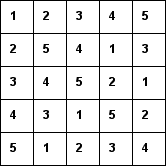
\includegraphics{./img/lat_quadrat.png}
\caption{Lateinisches Quadtrat}
\end{center}
\end{figure}

Daraus hat sich das heutige Sudoku entwickelt, das sich nicht nur bei Mathematikern großer Beliebtheit erfreut.